\documentclass[tikz, border=10mm]{standalone}
\usetikzlibrary{calc}
\usepackage{bm}% bold math
\def\pyramidwidth{1.0cm}
\def\pyramiddepth{0.5cm}
\def\pyramidheight{.35cm}
\def\levels{6}
\def\levelsep{0.05}
\usetikzlibrary{calc,shadings,shadows,fadings}
\usetikzlibrary{shadows.blur, positioning}
\usetikzlibrary{shapes.geometric} % Cylinder
\usetikzlibrary{shapes.symbols} 
\usetikzlibrary{shapes.callouts} 
\usetikzlibrary{shapes.misc} 
\usetikzlibrary{arrows.meta,bending,positioning} 
\begin{document}
	\sffamily
	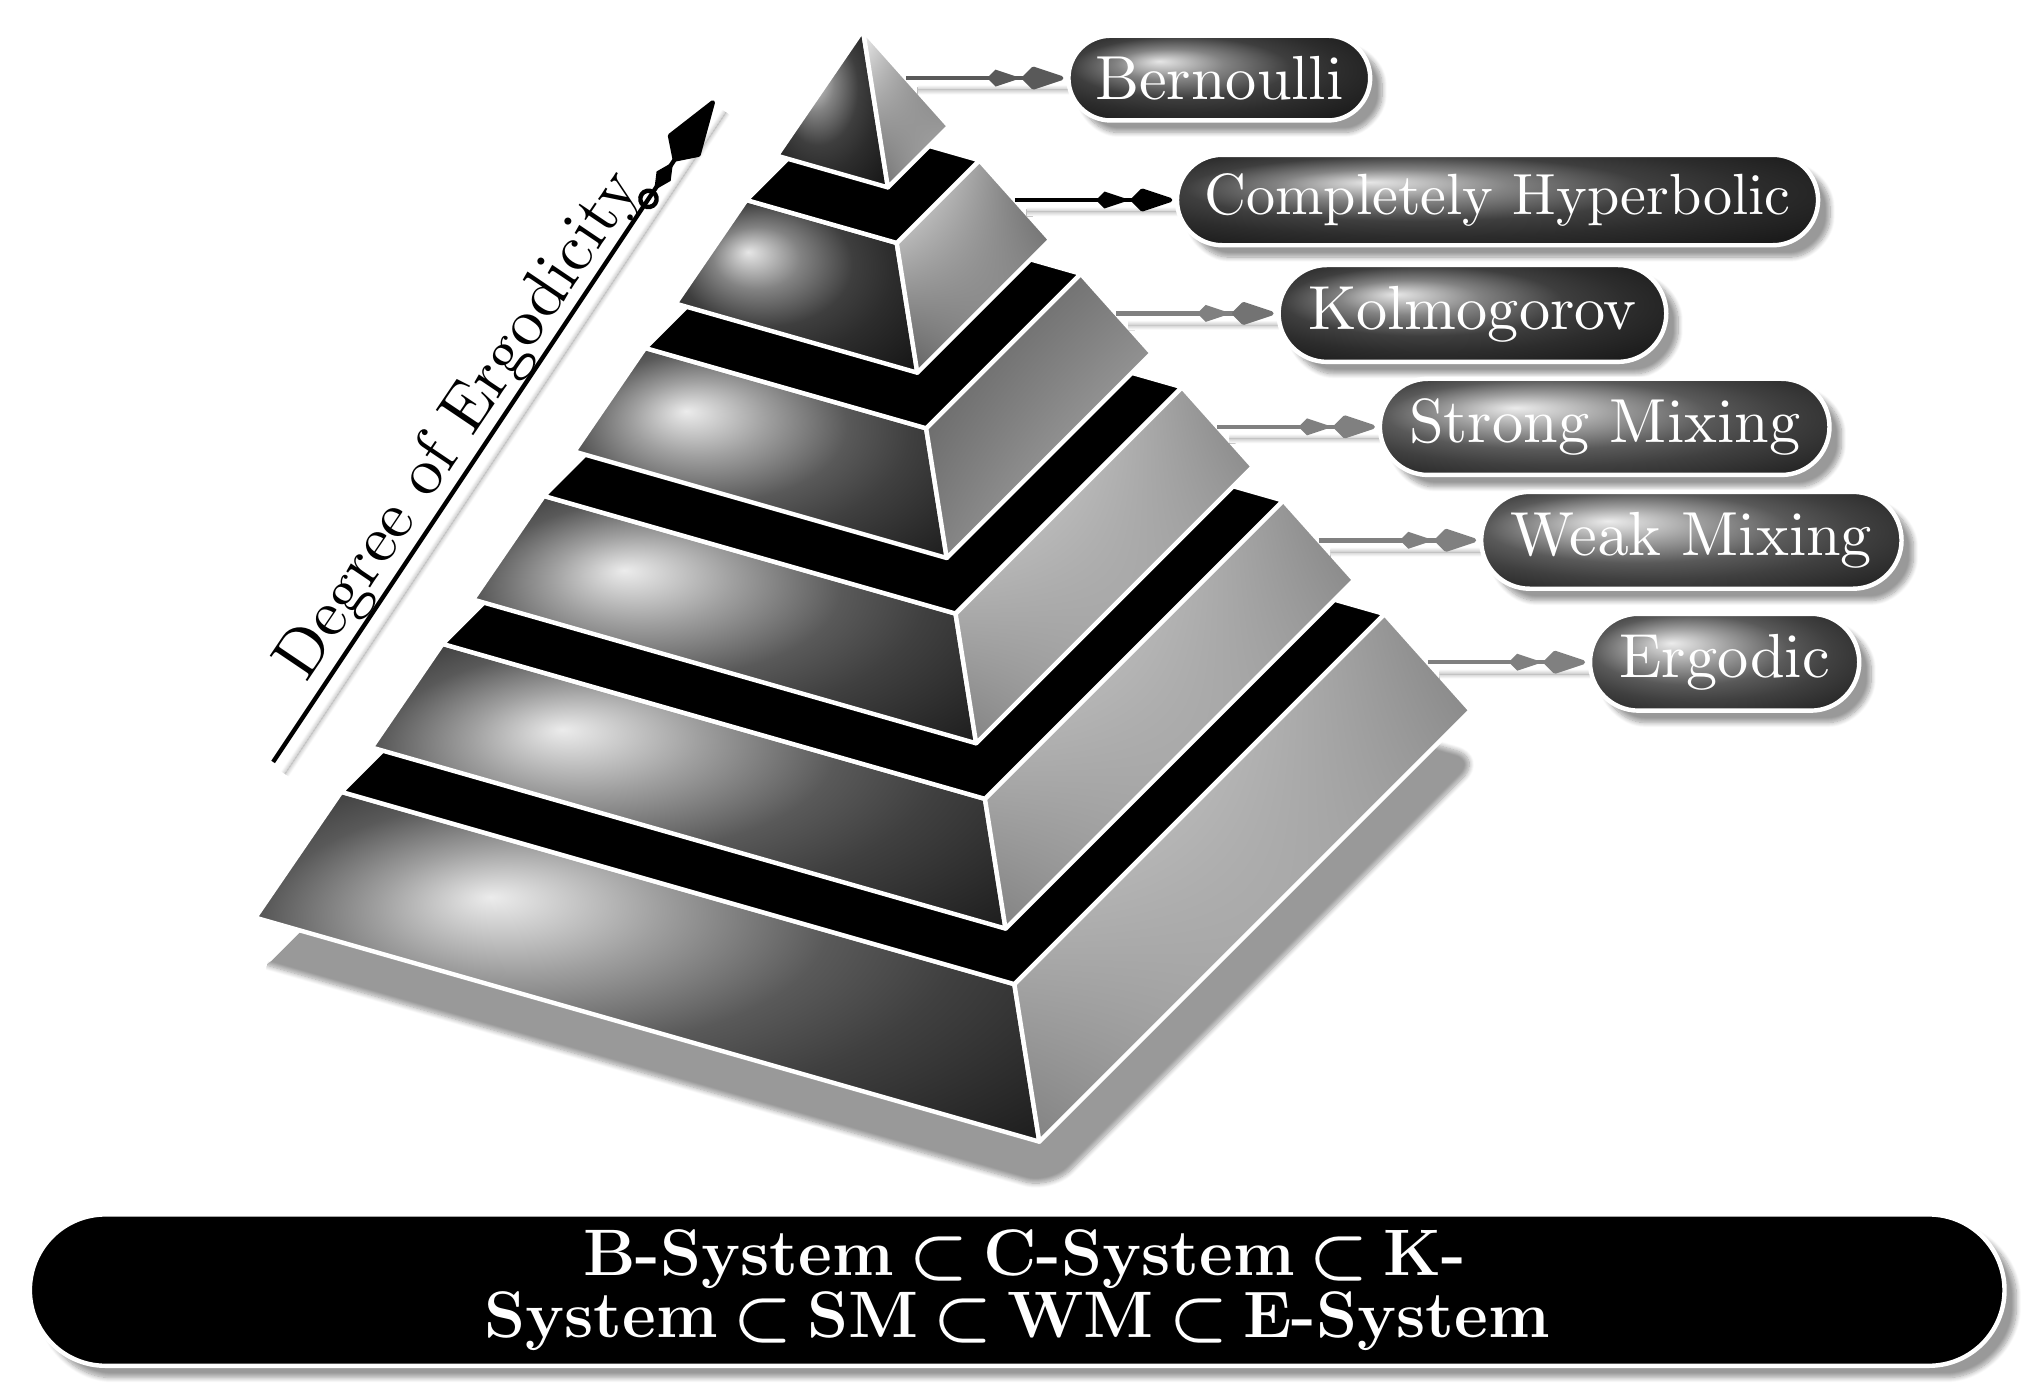
\begin{tikzpicture}[ line width=1pt, every node/.style={scale=3},
	level 1/.style={draw=white, ball color=blue},
	level 2/.style={ draw=white, ball color=red},
	level 3/.style={ draw=white, ball color= gray},
	level 4/.style={ draw=white, ball color=gray!90!black},
	level 5/.style={draw=white, ball color=gray},
	level 6/.style={draw=white, ball color=gray},
		x={(3.5mm,-1mm)}]
		
		\coordinate[alias=A1b] (A) at (0,0,0);
		\coordinate[alias=C1b] (C) at (\pyramidwidth,0,\pyramiddepth);
		\coordinate[alias=B1b] (B) at (0,0,\pyramiddepth);
		\coordinate[alias=D1b] (D) at (\pyramidwidth,0,0);
		\coordinate (H) at (\pyramidwidth/2,\pyramidheight,\pyramiddepth/2);
		\foreach \n in {A,B,C,D}{%
			\foreach \level[remember=\level as \lastlevel (initially 1)] in {2,...,\levels}{%
				\coordinate (\n\lastlevel t) at ($(\n)!\lastlevel/\levels-\levelsep/2!(H)$);
				\coordinate (\n\level b) at ($(\n)!\lastlevel/\levels+\levelsep/2!(H)$);}}
		\foreach \n in {A,B,C,D}{\coordinate (\n\levels t) at (H);}
		\foreach \level in {1,...,\levels}{%
			\foreach \i/\j in {D/A, A/B, B/C, C/D}{%
				\draw[level \level, line join=round] (\i\level b) -- (\j\level b) -- (\j\level t) -- (\i\level t) -- cycle;};
			\draw[level \level, line join=round] (A\level t) -- (B\level t) -- (C\level t) -- (D\level t) -- cycle;};
			
%%%%%%%%%%%%%%%%%%%%%%%%%%%%%%%%%%%%%%%%%%%%%%%%%%%%%%%%%%%%%%
%% First level
\path[%drop shadow={shadow scale=0.99, shadow xshift=.1ex, shadow yshift=-4ex, opacity=.5, fill=gray},
 blur shadow={shadow blur steps=10,
	shadow blur extra rounding=10pt, 
	shadow xshift=1ex,
	shadow yshift=-4ex}] (B1b) -- (C1b) -- (D1b) -- (A1b);		
\draw[line join=round, draw=white, ultra thick] (D1b) -- (A1b) -- (A1t) -- (D1t) -- cycle;
\draw[line join=round, draw=white, ultra thick] (A1b) -- (B1b) -- (B1t) -- (A1t) -- cycle;
\shade[line join=round, upper right=gray!10, lower left=gray, upper left=gray, lower right=gray, draw=white, ultra thick,ball color=gray] (B1b) -- (C1b) -- (C1t) -- (B1t) -- cycle;%F
\shade[line join=round, upper left=gray!10, lower right=gray!50, upper right=gray, lower left=gray, draw=white, ultra thick] (C1b) -- (D1b) -- (D1t) -- (C1t) -- cycle;
\shade[line join=round, lower right=black, upper right=black, lower left=black, upper left=black, draw=white, ultra thick] (A1t) -- (B1t) -- (C1t) -- (D1t) -- cycle;

%2nd
%\path[drop shadow={shadow scale=0.9, shadow xshift=.5ex, shadow yshift=-4ex, opacity=.5, fill=gray}] (B2b) -- (C2b) -- (D2b) -- (A2b);
\draw[line join=round, draw=white, ultra thick] (D2b) -- (A2b) -- (A2t) -- (D2t) -- cycle;
\draw[line join=round, draw=white, ultra thick] (A2b) -- (B2b) -- (B2t) -- (A2t) -- cycle;
\shade[line join=round, upper right=gray!10, lower left=gray, upper left=gray, lower right=gray, draw=white, ultra thick, ball color=gray] (B2b) -- (C2b) -- (C2t) -- (B2t) -- cycle;
\shade[line join=round, upper left=gray!10, lower right=gray!50, upper right=gray, lower left=gray, draw=white, ultra thick] (C2b) -- (D2b) -- (D2t) -- (C2t) -- cycle;
\shade[line join=round, lower right=black, upper right=black, lower left=black, upper left=black, draw=white, ultra thick] (A2t) -- (B2t) -- (C2t) -- (D2t) -- cycle;

%3rd
%\path[drop shadow={shadow scale=0.9, shadow xshift=.5ex, shadow yshift=-4ex, opacity=.5, fill=gray}] (B2b) -- (C2b) -- (D2b) -- (A2b);
\draw[line join=round, draw=white, ultra thick] (D3b) -- (A3b) -- (A3t) -- (D3t) -- cycle;
\draw[line join=round, draw=white, ultra thick] (A3b) -- (B3b) -- (B3t) -- (A3t) -- cycle;
\shade[line join=round, upper right=gray!10, lower left=gray, upper left=gray, lower right=gray, draw=white, ultra thick, ball color=gray] (B3b) -- (C3b) -- (C3t) -- (B3t) -- cycle;
\shade[line join=round, upper left=gray!10, lower right=gray!50, upper right=gray, lower left=gray, draw=white, ultra thick] (C3b) -- (D3b) -- (D3t) -- (C3t) -- cycle;
\shade[line join=round, lower right=black, upper right=black, lower left=black, upper left=black, draw=white, ultra thick] (A3t) -- (B3t) -- (C3t) -- (D3t) -- cycle;

%4th
%\path[drop shadow={shadow scale=0.9, shadow xshift=.5ex, shadow yshift=-4ex, opacity=.5, fill=gray}] (B4b) -- (C4b) -- (D4b) -- (A4b);
\draw[line join=round, draw=white, ultra thick] (D4b) -- (A4b) -- (A4t) -- (D4t) -- cycle;
\draw[line join=round, draw=white, ultra thick] (A4b) -- (B4b) -- (B4t) -- (A4t) -- cycle;
\shade[line join=round, upper right=gray!10, lower left=gray, upper left=gray, lower right=gray, draw=white, ultra thick, ball color=gray] (B4b) -- (C4b) -- (C4t) -- (B4t) -- cycle;
\shade[line join=round, upper left=gray!70!black, lower right=gray!50, upper right=gray, lower left=gray, draw=white, ultra thick] (C4b) -- (D4b) -- (D4t) -- (C4t) -- cycle;
\shade[line join=round, lower right=black, upper right=black, lower left=black, upper left=black, draw=white, ultra thick] (A4t) -- (B4t) -- (C4t) -- (D4t) -- cycle;

%5th
%\path[drop shadow={shadow scale=0.9, shadow xshift=.5ex, shadow yshift=-4ex, opacity=.5, fill=gray}] (B4b) -- (C4b) -- (D4b) -- (A4b);
\draw[line join=round, draw=white, ultra thick] (D5b) -- (A5b) -- (A5t) -- (D5t) -- cycle;
\draw[line join=round, draw=white, ultra thick] (A5b) -- (B5b) -- (B5t) -- (A5t) -- cycle;
\shade[line join=round, upper right=gray!10, lower left=gray!90!black, upper left=gray!90!black, lower right=gray!70!black, draw=white, ultra thick, ball color=gray!70!black] (B5b) -- (C5b) -- (C5t) -- (B5t) -- cycle;
\shade[line join=round, upper left=gray!10, lower right=gray!70, upper right=gray!70!black, lower left=gray!70!black, draw=white, ultra thick] (C5b) -- (D5b) -- (D5t) -- (C5t) -- cycle;
\shade[line join=round, lower right=black, upper right=black, lower left=black, upper left=black, draw=white, ultra thick] (A5t) -- (B5t) -- (C5t) -- (D5t) -- cycle;

%6th
%\path[drop shadow={shadow scale=0.9, shadow xshift=.5ex, shadow yshift=-4ex, opacity=.5, fill=gray}] (B5b) -- (C5b) -- (D5b) -- (A5b);
\draw[line join=round, draw=white, ultra thick] (D6b) -- (A6b) -- (A6t) -- (D6t) -- cycle;
\draw[line join=round, draw=white, ultra thick] (A6b) -- (B6b) -- (B6t) -- (A6t) -- cycle;
\shade[line join=round, upper right=gray!10, lower left=gray, upper left=gray, lower right=gray, draw=white, ultra thick, ball color=gray!70!black] (B6b) -- (C6b) -- (C6t) -- (B6t) -- cycle;
\shade[line join=round, upper left=gray!10, lower right=gray!50, upper right=gray!70!black, lower left=gray!70!black, draw=white, ultra thick] (C6b) -- (D6b) -- (D6t) -- (C6t) -- cycle;
\shade[line join=round, lower right=gray!10, upper right=gray, lower left=gray, upper left=gray, draw=white, ultra thick] (A6t) -- (B6t) -- (C6t) -- (D6t) -- cycle;	

%%%%%%%%%%%%%%%%%%%%%%%%%%%%%%%%%%%%%%%%%%%%%%%%%%%%%%%%%%%%%%
%		\begin{scope}[every node/.style={rotate=-16, xslant=.1, above, inner sep=3pt, font=\bfseries, text=white}]
%			\node[scale=4] at ($(B1b)!.5!(C1b)$) {$\bm\lambda=0$};
%			\node[scale=3] at ($(B2b)!.5!(C2b)$) {$\bm\lambda = 0$};
%			\node[scale=2] at ($(B3b)!.5!(C3b)$) {$\bm\lambda \geq 0$};
%			\node[scale=1.4] at ($(B4b)!.5!(C4b)$) {$\bm\lambda > 0$};
%			\node[scale=1.4] at ($(B5b)!.5!(C5b)$) {$\bm \lambda > 0$};
%			\node[scale=1.2] at ($(B6b)!.5!(C6b)$) {$\bm\lambda \gg 0$};
%		\end{scope}
		
%%%%%%%%%%%%%%%%%%%%%%%%%%%%%%%%%%%%%%%%%%%%%%%%%%%%%%%%%%%%%%
\begin{scope}[x=2cm]
\draw[gray!70!black, arrows = -{Kite[]Kite[length=6mm, round,  gray!70!black]}, ultra thick, blur shadow={shadow blur steps=10,
	shadow blur extra rounding=2pt, 
	shadow xshift=1ex,
	shadow yshift=-1ex}] ($(D6b)!.5!(D6t)$) -- +(1,0) node[right, text=white, draw=white, text=white, rounded rectangle, ball color=gray!70!black, shading=ball, scale=0.75, shading=ball, blur shadow={shadow blur steps=10,
	shadow blur extra rounding=2pt, 
	shadow xshift=1ex,
	shadow yshift=-1ex}] {Bernoulli};

\draw[black, arrows = -{Kite[]Kite[length=6mm, round,  black]},ultra thick, blur shadow={shadow blur steps=10,
	shadow blur extra rounding=2pt, 
	shadow xshift=1ex,
	shadow yshift=-1ex}] ($(D5b)!.5!(D5t)$) -- +(1,0) node[right, text=white, scale=0.7, draw=white, rounded rectangle, rounded rectangle west arc=convex, draw, fill=gray!20, ball color=gray!70!black, shading=ball, blur shadow={shadow blur steps=10,
	shadow blur extra rounding=2pt, 
	shadow xshift=1ex,
	shadow yshift=-1ex}] {Completely Hyperbolic};

\draw[gray, arrows = -{Kite[]Kite[length=6mm, round,  gray!90!black]}, ultra thick, blur shadow={shadow blur steps=10,
	shadow blur extra rounding=2pt, 
	shadow xshift=1ex,
	shadow yshift=-1ex}] ($(D4b)!.5!(D4t)$) -- +(1,0) node[right, scale=0.75, text=white, draw=white, rounded rectangle, ball color=gray!70!black, shading=ball, blur shadow={shadow blur steps=10,
	shadow blur extra rounding=2pt, 
	shadow xshift=1ex,
	shadow yshift=-1ex}] {Kolmogorov};

\draw[gray, arrows = -{Kite[]Kite[length=6mm, round,  gray]},% -{Stealth[length=5mm,round, gray]},
ultra thick, blur shadow={shadow blur steps=10,
	shadow blur extra rounding=2pt, 
	shadow xshift=1ex,
	shadow yshift=-1ex}] ($(D3b)!.5!(D3t)$) -- +(1,0) node[right, scale=0.75, text=white, draw=white, rounded rectangle, ball color=gray, shading=ball, blur shadow={shadow blur steps=10,
	shadow blur extra rounding=2pt, 
	shadow xshift=1ex,
	shadow yshift=-1ex}] {Strong Mixing};

\draw[gray, arrows = -{Kite[]Kite[length=6mm, round,  gray]},% -{Stealth[length=5mm,round, red]},
 ultra thick, blur shadow={shadow blur steps=10,
	shadow blur extra rounding=2pt, 
	shadow xshift=1ex,
	shadow yshift=-1ex}] ($(D2b)!.5!(D2t)$) -- +(1,0) node[right, scale=0.75, text=white, draw=white, rounded rectangle, ball color=gray, shading=ball, blur shadow={shadow blur steps=10,
	shadow blur extra rounding=2pt, 
	shadow xshift=1ex,
	shadow yshift=-1ex}] {Weak Mixing};

\draw[gray, arrows = -{Kite[]Kite[length=6mm, round,  gray]}, ultra thick, blur shadow={shadow blur steps=10,
	shadow blur extra rounding=2pt, 
	shadow xshift=1ex,
	shadow yshift=-1ex}] ($(D1b)!.5!(D1t)$) -- +(1,0) node[right, scale=0.75, text=white, draw=white, rounded rectangle, ball color=gray, shading=ball, blur shadow={shadow blur steps=10,
	shadow blur extra rounding=2pt, 
	shadow xshift=1ex,
	shadow yshift=-1ex}] {Ergodic};
\end{scope}

\draw[black, arrows = -{Circle[open]Diamond[]Kite[length=10mm, round,  black]}, ultra thick, blur shadow={shadow blur steps=10,shadow blur extra rounding=2pt, shadow xshift=1ex,shadow yshift=-1ex}] (-15,-5)--(1,5)
node[left, scale=0.8, text=black, rotate=56, xshift=-3ex, yshift=1ex] {Degree of Ergodicity};

\draw (12,-8) node[below, scale=0.55, text=black, draw=white, rounded rectangle, ultra thick, 
%ball color=black, shading=ball, 
blur shadow={shadow blur steps=10, shadow blur extra rounding=2pt, shadow xshift=1ex, shadow yshift=-1ex},
 fill=black,align=center, text width=14.5cm, text height=10pt
 ] {\Large \textbf{ 
 	\color{white} B-System 
 	\color{white} $\bm\subset$ \color{white!50} C-System 
 	\color{white}$\bm\subset$ \color{white!50} K-System 
 	\color{white}$\bm\subset$ \color{white!50} SM 
 	\color{white}$\bm\subset$ \color{white!50} WM \color{white}$\bm\subset$ \color{white!50} E-System}};
	\end{tikzpicture}
%	\begin{tikzpicture}
%		\path[draw=red]circle (5pt) (0,0) -- (0.5,0.5) -- (2,1)circle (10pt);
%	\end{tikzpicture}
\end{document}